% Tento soubor nahraďte vlastním souborem s obsahem práce.
%=========================================================================
% Autoři: Michal Bidlo, Bohuslav Křena, Jaroslav Dytrych, Petr Veigend a Adam Herout 2019

% Pro kompilaci po částech (viz projekt.tex), nutno odkomentovat a upravit
%\documentclass[../projekt.tex]{subfiles}
%\begin{document}

\chapter{Úvod}
Podpis je jednou z~nejstarších metod používanou pro ověření totožnosti, určení autorství či udělení právního souhlasu.
Dodnes se stále používá pro jeho uživatelskou přívětivost a akceptovatelnost zákonem.
S technologiemi dnešní doby není problémem tento podpis digitalizovat a používat ho k automatizované autentizaci.
V~této práci půjde o oklamání automatizované autentizace pomocí replikace vlastnoručního podpisu.
Autentizace spadá pod obor zvaný biometrie, která se zabývá analýzou biologických a behaviorálních charakteristik. 
U~podpisu lze pak analyzovat dvě skupiny charakteristik písma, a to statické a dynamické. 
Statické charakteristiky lze extrahovat z hotového podpisu, oproti tomu dynamické musí být zaznamenávány v průběhu podpisu.

Podpis je v~praxi stále nejpoužívanější způsob autentizace v právních, komerčních či jiných oblastech. 
Pro autentizaci se používají a zkoumají především dynamické vlastnosti písma, jelikož je mnohem těžší je replikovat, a tedy zajišťují větší míru bezpečnosti.
Podaří-li se důvěryhodně vlastnoruční podpis replikovat, bude možné pomocí falzifikátu obejít bezpečnostní zabezpečení. 
To představuje velké bezpečnostní riziko a nutnost upravení dosavadních bezpečnostních metod pro autentizaci. 


%TOLE JE SPIS ABSTRAKT
%Bude třeba sestavit snímací zařízení pro získaní potřebných parametrů podpisu.
%Ze statických parametrů budeme snímat tvar i tloušťku čar a celkový vzhled podpisu. 
%Z dynamických parametrů budeme snímat tlak, sklon a průběh tahů. 
%Získané data je potřeba vhodným způsobem zpracovat a provést potřebné výpočty. 
%Upravená data je poté potřeba převést do instrukcí pro mechanickou paži, která je použita k replikaci podpisu. 
%Výsledný podpis bude porovnáván s vlastnoručním podpisem. Cílem je co nejvíce se přiblížit vlastnoručnímu podpisu.

%\section{Představení tématu}
%\section{Cíle práce}

%\section{Struktura práce}

\chapter{Teoretické základy}
Pro plné pochopení problematiky je potřeba představit základy z~několika odvětví. 
V~této části budou shrnuty všechny potřebné informace. 

\section{Pojmy}\label{sec:pojmy}
\begin{itemize} 
  \item \textbf{Biometrie} --- automatizované rozpoznávání osob na základě jejich charakteristických biologických a behaviorálních rysů.~\cite{DrahanskýMartin2011} % parafráze biometrie (str. 13) / Biometric identification - parafráze (str 3)
  \item \textbf{Biologické autentizační metody} --- zkoumají biologické charakteristiky člověka, s~jimiž se narodí. Tyto charakteristiky má každý člověk unikátní a jsou neměnitelné. Patří mezi ně například otisky prstů, skeny sítnice či duhovky.  
  \item \textbf{Behaviorální autentizační metody} --- porovnávají behaviorální charakteristiky související s~chováním člověka. Lze například porovnávat, jakým způsobem jedinec mluví nebo jak pohybuje očima.
  \item \textbf{Statické parametry písma} --- jde o~parametry, které nezahrnují informace o~procesu psaní podpisu. Patří mezi ně například tvar a vzhled písma, umístění podpisu na stránce či tloušťka čar.
  \item \textbf{Dynamické parametry písma} --- tyto parametry se vztahují k~samotnému průběhu psaní podpisu. Například rychlost psaní, akcelerace, tlak nebo průběh tahů.
\end{itemize}

Dále je potřeba si ujasnit tyto tři pojmy:
\begin{itemize}
  \item \textbf{Verifikace} --- potvrzení totožnosti jedince porovnáním poskytnutého vzoru s referenčním vzorem dané osoby uloženého v databázi, % |
  za kterou se vydává. Probíhá tedy principem one-to-one.                                                                                     % |
  \item \textbf{Identifikace} --- určení identity předem neznámého jedince.                                                                       % |
  Jde tedy o přikládání poskytnutého vzoru ke všem vzorům v databázi, tedy princip one-to-many.                                                % |
  \item \textbf{Autentizace} --- je proces, vyskytující se především u přístupových systému.                                                      % |
  Může se u ní jednat při verifikaci i identifikaci.                                                                                            % V
  Výsledkem bývá získání nějakého statusu, například získání určitých oprávnění.~\cite{Scurek2015}                                                        % Biometrické technologie (str. 4-5) https://www.fbi.vsb.cz/export/sites/fbi/060/.content/galerie-souboru/studijni-materialy/BiometrickeTechnologie.pdf
\end{itemize}


\section{Definice podpisu a jeho charakteristiky}
Definice podpisu je z~pohledu zákona poněkud problematická. 
Podpis jako takový není v~zákoně nijak přímo definován. 
Obecně je ale bráno za podpis vlastnoruční uvedení jména a příjmení, nebo jiného jedinečného a nezaměnitelného označení.~\cite{Fulsoft2023} % parafraze https://www.fulsoft.cz/33/komentar-zakona-89-2012-sb-obcansky-zakonik-561-uniqueidmRRWSbk196FNf8-jVUh4EtuvCojfP1Dmx8t50X_QR_yU_dtwjPItMA/

Podpis patří z části ke statickým a z části k dynamickým biometrickým vlastnostem.
Pokud se uchovává pouze výsledek psaní podpisu, lze z něj extrahovat pouze statické parametry.
Pro snímání dynamických parametrů je nutné snímat podpis v průběhu jeho psaní.
Těchto parametrů je mnoho, ale pro zjednodušení se jich používá jen omezené množství.

Dynamické vlastnosti poskytují více informací a umožňují lépe identifikovat neoprávněného uživatele pokoušejícího se podpis falzifikovat.    % V
K zaznamenání těchto dynamických vlastností je avšak zapotřebí tablet a speciální pero, které při psaní ukládá relevantní parametry.~\cite{DrahanskýMartin2011}  % parafráze Biometrie (str 233)

\section{Biometrická autentizace}
Biometrie je jedním ze tří hlavních kategorií autentizace.
Autentizovat se můžeme pomocí toho:

\begin{itemize}
  \item co vlastníme --- identifikační doklady, karty, čipy\ldots   % ? | 
  \item co známe --- přihlašovací jména, hesla\ldots                % ? |
  \item čím fyzicky jsme --- otisky prstu, tvář, oči, podpis\ldots~\cite{RakRoman2008}% ? V
\end{itemize}                                                   % parafráze Biometrie a identita člověka (str 89) 
Biometrie spadá do třetí kategorie, tedy čím fyzicky jsme. 
\newline

Biometrická autentizace probíhá na základě biologických a behaviorálních charakteristik člověka\ref{sec:pojmy}. 
Obě tyto skupiny znaků jsou pro každého člověka unikátní a nezaměnitelné. To je důvodem, proč je lze využít k~autentizaci.
Existuje spousta biometrických metod pro autentizaci, kupříkladu otisk prstu, rozpoznání obličeje, sken duhovky či sítnice, nebo pomocí používání myši. 
Každá tato metoda má své výhody a nevýhody, zejména se hodnotí přesnost, cena, komfort používání, stálost a velikost vzorku. % ?
%Tato práce se zaměřuje na autentizaci pomocí podpisu.

Biometrický systém je v informačních technologiích postup pro rozpoznávání vzorů lidských vlastností.       % |
Existuje spoustu různých cest, kterými lze biometrické systémy napadnout.                                   % |
V~rámci této práce se zaměříme na senzor, jenž je první komponentou biometrického systému~\ref{fig:biometricky_system}.% V
Tomuto senzoru budeme předkládat falešné biometriky, v~našem případě falešný podpis.~\cite{DrahanskýMartin2011}% parafráze Biometrie (str 78)

\begin{figure}[h]
  \centering
  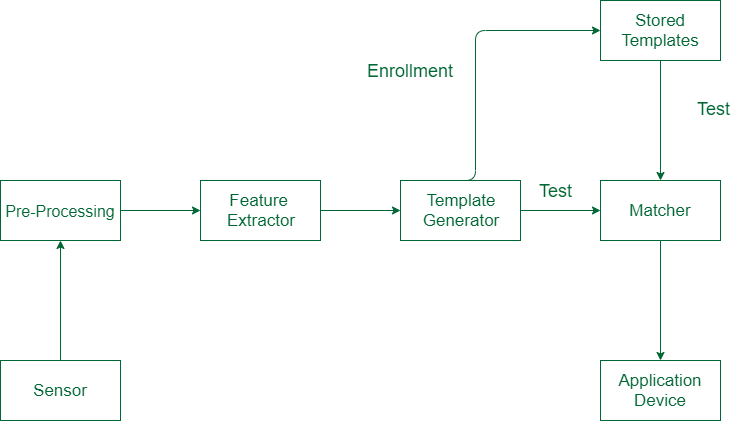
\includegraphics[width=0.5\textwidth]{obrazky-figures/biometricky_system.png}
  \caption{Biometrický systém~\cite{geeksforGeeks2022}}  % https://www.geeksforgeeks.org/biometric-system-architecture/
  \label{fig:biometricky_system}
\end{figure}

\newpage

\section{Parametry podpisu}
V~rámci této práce budou snímány následující parametry:
\begin{itemize}
  \item \textbf{Celkový vzhled podpisu}
  \item \textbf{Pohyb pera}, ze kterého bude vypočítán celkový průběh podpisu, především pak pozice pera a rychlost psaní čar. 
  \item \textbf{Sklon pera} 
  \item \textbf{Tlak}
\end{itemize}
Kombinací těchto nasnímaných parametrů bude možné dostatečně věrohodně napodobit původní vlastnoruční podpis. 

\section{Rozpoznávání falzifikátů}
Rozpoznání falzifikátu probíhá u statického a dynamického podpisu odlišně. 
Následující text se bude týkat postupu, který sdílejí.

Falzifikáty jsou vyhodnoceny na základě porovnávání uloženého vzorku v~databázi s~podpisem, kterým se daný člověk pokouší autentizovat.
Výsledkem takového porovnávání je určité procento shody parametrů.
Referenční podpis je zprůměrován z~několika vzorků, aby došlo k~potlačení náhodných jevů.~\cite{VUT2009} %  parafraze zav_prace 17183 2.3
Tyto vzorky jsou poskytnuté danou osobou při registraci do systému.

\begin{figure}[h]
  \centering
  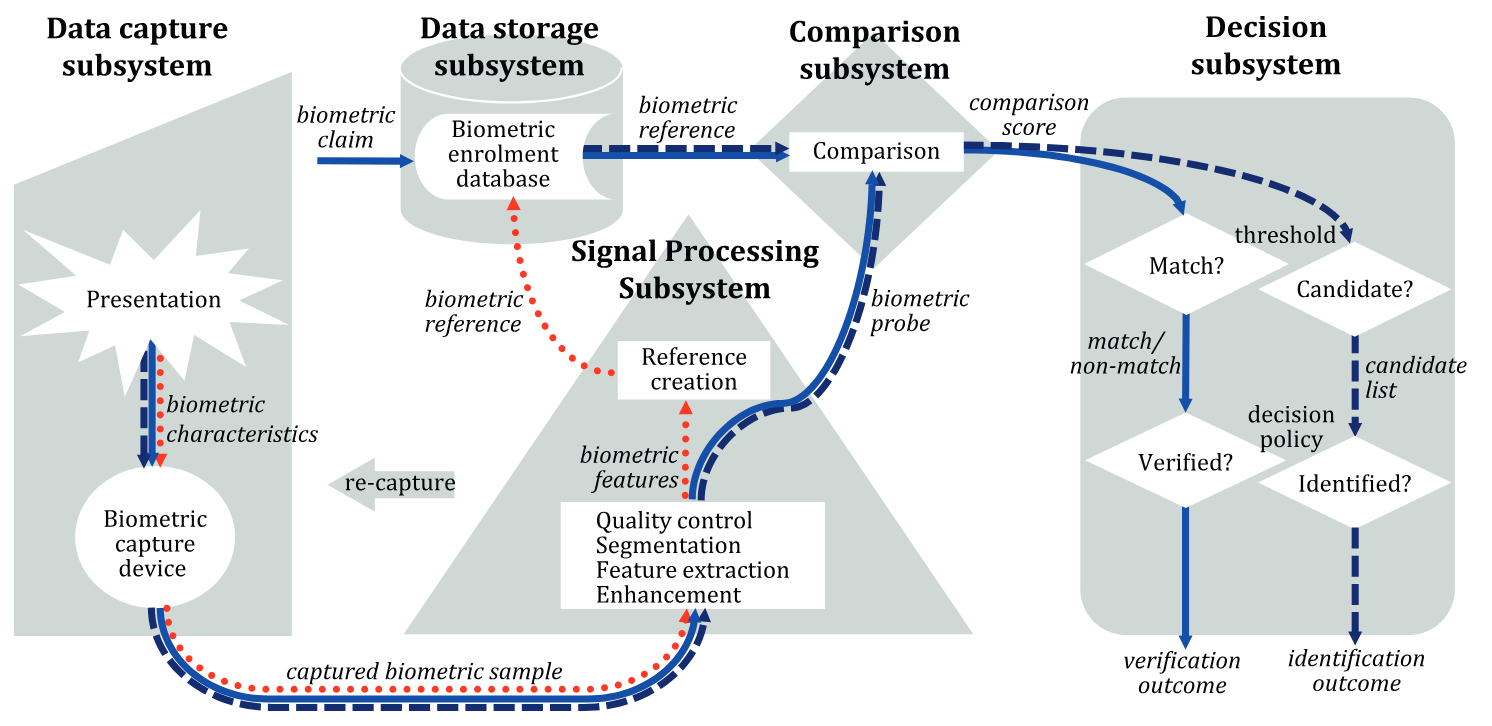
\includegraphics[width=0.5\textwidth]{obrazky-figures/proces_autentizace.png}
  \caption{Průběh autentizace~\cite{ISOIEC19795-1_2021}}
  \label{fig:proces_autentizace} % ISO/IEC 19795-1 str 7.
\end{figure}

Obě tyto skupiny charakteristik jsou ovlivňovány jak fyzickým, tak i psychologickým stavem člověka v~době podpisu.
To znamená, že ani též osobě se nepovede dvakrát úplně totožný podpis.
Pokud jsou podpisy naprosto stejné, nejspíše půjde právě o padělek.

Porovnávací algoritmus extrahuje důležité parametry podpisu, které poté porovnává s~referenčním vzorem. 
Následně je vypočteno celkové procento shody podpisů a na jeho základě je autentizace úspěšná, či nikoli.
Je přitom důležité, aby algoritmus měl určenou správnou procentuální hodnotu shody. 

Pokud by bylo procento shody špatně zvoleno, došlo by k jednomu ze dvou problémů, a to zvýšení následujících:
\begin{itemize}
  \item \textbf{míra falešných odmítnutí (FRR)} --- míra neúspěšných autentizací, které měly být úspěšné.
  \item \textbf{míra falešných akceptací (FAR)} --- míra úspěšných autentizací, které měly být neúspěšné.
\end{itemize}

Pokud je procento shody nastaveno právě v bodě protnutí těchto dvou křivek (viz~\ref{fig:FAR_FRR}), nazýváme ho rovnoměrná míra chybovosti (EER), 

\begin{figure}[h]
  \centering
  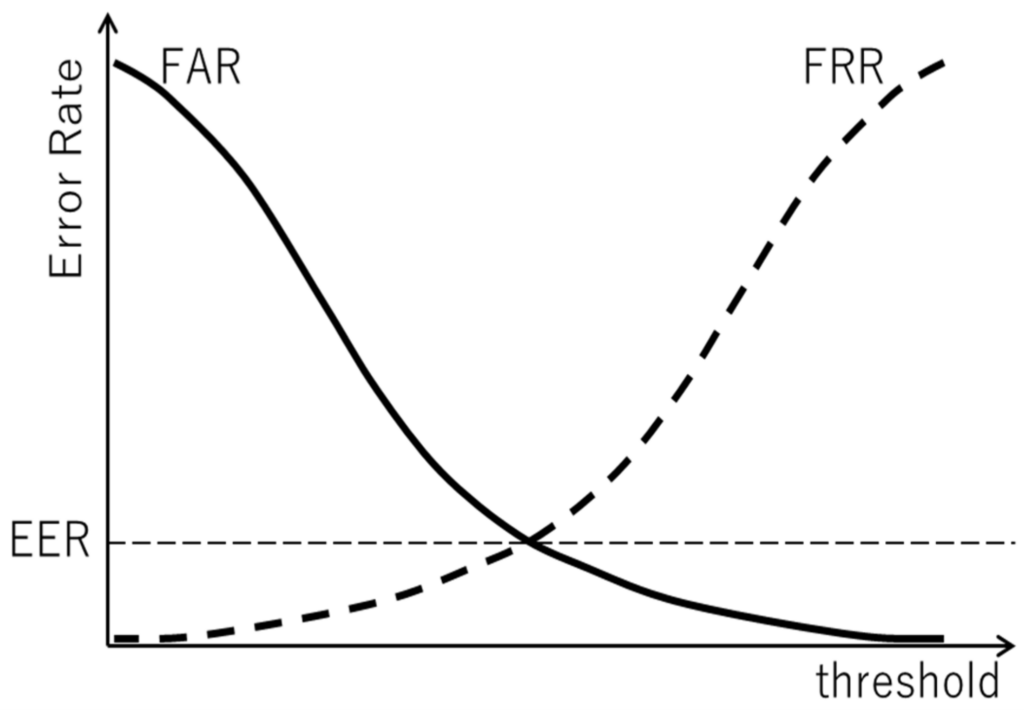
\includegraphics[width=0.5\textwidth]{obrazky-figures/FAR_FRR.png}
  \caption{Rovnoměrná míra chybovosti (EER), míra falešných odmítnutí (FRR) a míra falešných akceptací (FAR)~\cite{cursorinsight_frr_fa}} % https://www.cursorinsight.com/post/943/what-you-need-to-know-about-frr-and-far
  \label{fig:FAR_FRR}
\end{figure}

\newpage

\section{Off-line systémy pro verifikaci}
Off-line systémy pro verifikaci se rozumí systémy, které ověřují totožnost na základě statického podpisu, tedy psaného na papír.  % |
Obraz podpisu je naskenován či nasnímán kamerou a tím je získán digitální obraz podpisu.                                          % |
Tento obraz je následně porovnáván v databázi s referenčním podpisem.                                                             % |
Tato metoda je, při existenci skenovacích a kopírovacích zařízení, nepoužitelná, co se týče automatizovaného zpracování, jelikož je statický podpis náchylný na falzifikaci.~\cite{RakRoman2008}% Parafráze Biografie a identita člověka (str 440)

Verifikace probíhá ve třech fázích --- předzpracování, extrakce biometrických charakteristik a vyhodnocování. % |
V předzpracování projde naskenovaný obraz podpisu prahováním, vyhlazováním, normalizací a zjednodušováním.    % |
Následně jsou extrahovány biometrické charakteristiky podpisu,                                                % |
například hustota vodorovných a svislých čar nebo vektory ohraničené oblasti.                                 % |
Vyhodnocování je založeno na extrahovaných charakteristikách a jejich vektorech.                              % V
Může být provedeno porovnáním významových bodů, klasifikátorem sousedů nebo  pomocí neuronové sítě.\cite{RakRoman2008}% Parafráze Biometrie a identita člověka (strana 441 442 443) - nebo https://theses.cz/id/odwy80/BP_Vchov.pdf

\begin{figure}[h]
  \centering
  \begin{minipage}{0.3\textwidth}
    \centering
    
\includegraphics[width=\textwidth]{obrazky-figures/placeholder.pdf}
    \caption{Předzpracovaný podpis.}
    \label{fig:first-image}
  \end{minipage}\hfill
  \begin{minipage}{0.3\textwidth}
    \centering
    
\includegraphics[width=\textwidth]{obrazky-figures/placeholder.pdf}
    \caption{Extrahované parametry.}
    \label{fig:second-image}
  \end{minipage}\hfill
  \begin{minipage}{0.3\textwidth}
    \centering
    
\includegraphics[width=\textwidth]{obrazky-figures/placeholder.pdf}
    \caption{Vyhodnocová- ní}
    \label{fig:third-image}
  \end{minipage}
\end{figure}


\section{On-line systémy pro verifikaci} 
On-line systémy na rozdíl od off-line neporovnávají pouze výsledek podpisu, ale i data o jeho průběhu. % |
Důležité zde jsou parametry jako změny rychlosti či tlaku a celkový průběh psaní podpisu.              % |
K nasnímání těchto parametrů je potřeba tablet a speciální pero, které takové snímání umožní.          % |
Na rozdíl od statických parametrů, které lze snáze odpozorovat a napodobit                             % |
nebo pomocí technologií jinak replikovat, je dynamické parametry nemožné zfalšovat člověkem.           % V
Falzifikát lze vytvořit pomocí stroje, k čemuž je ale potřeba nasnímat pohyb ruky podepisujícího.~\cite{VaccaJohnR2007}% parafráze Biometric verification (str. 170)

\begin{figure}[h]
  \centering
  \begin{minipage}{0.45\textwidth}\label{fig:first-image}
      \centering
      
\includegraphics[width=\textwidth]{obrazky-figures/placeholder.pdf}
      \caption{Vzhled dynamického podpisu.}
  \end{minipage}\hfill
  \begin{minipage}{0.45\textwidth}\label{fig:second-image}
      \centering
      
\includegraphics[width=\textwidth]{obrazky-figures/placeholder.pdf}
      \caption{Graf dynamických parametrů podpisu v~čase.}
  \end{minipage}
\end{figure}

\section{Normy biometrické identifikace pomocí podpisu}

Vytvoření norem mělo velký pozitivní dopad na rozšíření biometrických systémů.                                                % |
Jde například o normy určující, jakým způsobem mají být biometrická data ukládána či jakým způsobem dochází k jejich vyměně.  % | 
Tyto normy přispěly k větší interoperabilitě jednotlivých komponent biometrických systémů.                                    % V
To znamená, že lze jeden komponent vyměnit za stejný od jiného výrobce a neměl by být problém s kompatibilitou.~\cite{DrahanskýMartin2011}% parafraze Biometrie str. 61
\newline 

\noindent
Normy obecně přinášejí několik zásadních výhod:
\begin{itemize}
  \item Interoperabilita --- Umožňují výměnu dat mezi různými systémy a zařízeními bez ztráty integrity nebo kompatibility.
  \item Bezpečnost --- Standardizované formáty zajišťují ochranu citlivých dat a minimalizují riziko neoprávněného přístupu.
  \item Spolehlivost --- Poskytují jednotné metody pro ukládání a zpracování dat, což zvyšuje přesnost a důvěryhodnost biometrických systémů.
  \item Právní jistota --- Splnění norem často znamená, že technologie odpovídá požadavkům právních a regulačních předpisů.
\end{itemize}

Autentizace vlastnoručním podpisem spadá pod několik norem, zaměřující se například na zachycení a uložení dat o podpisu, nebo způsob, jakým se tato data budou vyměňovat. 
Mezi nejdůležitější patří:

\subsection*{ISO/IEC Normy}
\begin{itemize}
  \item \textbf{ISO/IEC 19794-1:2011 (Framework)}: 
  Definuje obecný formát pro ukládání a používání biometrických dat, konvenci pojmenování datových struktur a podobně.\cite{iso19794-1_2011} % parafraze ISO/IEC 19794-1:2011 str. 1

  \item \textbf{ISO/IEC 30107-3:2017 (Biometric Presentation Attack Detection)}: 
  Tato norma se zabývá technikami pro automatickou detekci prezentačních útoků.~\cite{ISO/IEC30107-3_2017} % parafraze ISO/IEC 30107-3:2017 str. 1

  \item \textbf{ISO/IEC 19794-7:2021 (Signature/sign time series data)}:
  Specifikuje formát pro ukládání a výměnu dat pro dynamické podpisy. 
  Formát lze vidět na obrázku~\ref{fig:norms_table}. 
  Verze 2021 je novější verze té stejné normy z roku 2007.~\cite{ISOIEC19794-7_2021} % parafraze ISO/IEC 19794-7:2021 str. 1
\end{itemize}

\begin{figure}[h]
  \centering
  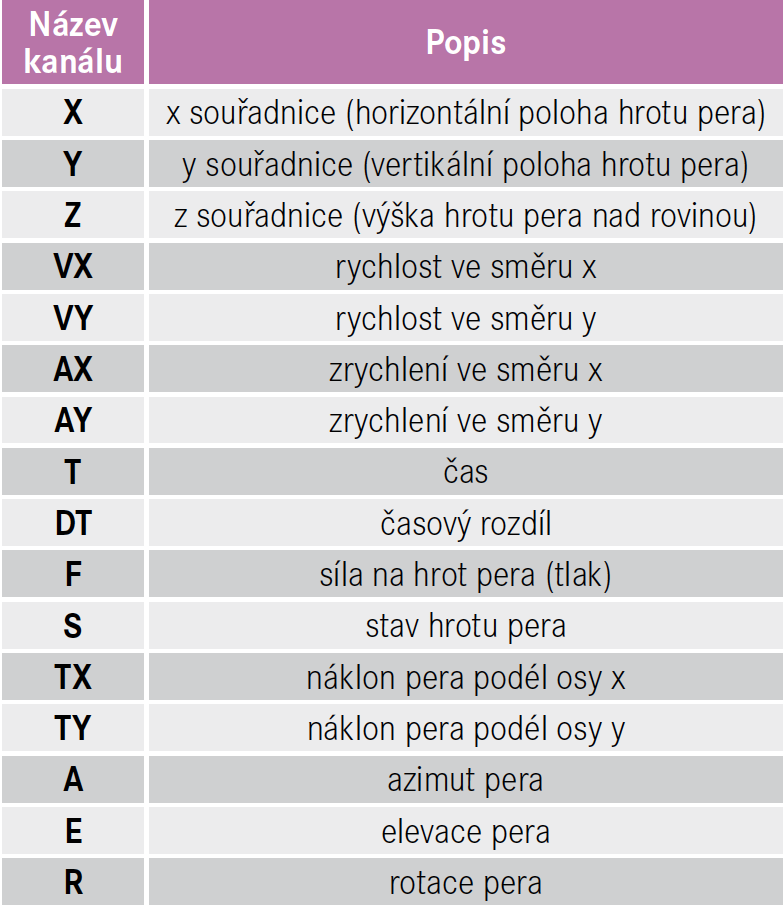
\includegraphics[width=0.5\textwidth]{obrazky-figures/normy.png}
  \caption{Struktura zaznamenávaných dat daná normou ISO/IEC 19794-7:2021.~\cite{DSM2021}} % https://dsm.tate.cz/cs/2021/dsm-3-2021/vlastnorucni-podpis-a-informacni-systemy-necekane-spojeni?utm_source=chatgpt.com
  \label{fig:norms_table}
\end{figure}

\newpage

\subsection*{ANSI/INCITS Normy}
\begin{itemize}
  \item \textbf{ANSI/INCITS 395-2005 (Signature/Sign Data)}  
  Definuje obecný formát pro výměnu dat digitalizovaného podpisu. Díky své obecnosti lze použít v široké škále aplikací.~\cite{ANSI_INCITS_395_2005} % parafraze ANSI/INCITS 395-2005 str. 1
  
  \item \textbf{ANSI/INCITS 398-2005 (Common Biometric Exchange Format Framework)}  
  Definuje soubor datových prvků potřebných k zajištění univerzální podpory různých biometrických technologií a stanovuje požadavky pro zajištění vzájemné kompatibility.~\cite{DrahanskýMartin2011} % parafraze biometrie str. 69
\end{itemize}

Existuje spousta dalších norem týkajících se jak biometrie, jiných biometrických metod či přímo digitálního podpisu.                % |
Kromě již zmíněných organizací existují další organizace zabývající se normami pro biometrii.                                      % V
Například NIST, působící na poli biometrických databází, TCSEC a Common Criteria, obojí zabývající se biometrií v rámci bezpečnosti.~\cite{DrahanskýMartin2011}% Biometrie str. 68-69

Normy v oblasti biometrického podpisu tvoří klíčový základ pro spolehlivé a bezpečné využití těchto technologií v praxi.


\chapter{Analýza současných řešení}

V současné době nabývají na významu biometrické systémy založené na využití vlastnoručních podpisů. 
Tyto systémy se úspěšně používají například v oblasti bankovnictví, elektronického obchodu, správy elektronických dokumentů a dalších oblastech, kde je potřeba provést autentizaci jedince. 

Existují dva přístupy k autentizaci uživatelů.
První je založena na statických parametrech („off-line“) --- zahrnuje rozpoznání podpisu osoby na základě analýzy jeho vzhledu.
Druhý je pak založen na dynamických parametrech („on-line“) --- zahrnuje čtení a rozpoznávání informací o dynamice psaní vlastnoručního podpisu.~\cite{9306154} % parafraze E. S. Anisimova and I. V. Anikin, "Finding a Rational Set of Features for Handwritten Signature Recognition," 2020 Dynamics of Systems, Mechanisms and Machines (Dynamics), Omsk, Russia, 2020, pp. 1-6, doi: 10.1109/Dynamics50954.2020.9306154.

Ne všechny údaje (viz obrázek~\ref{fig:norms_table}) jsou součástí každého podpisového řešení. 
Kromě dat získaných přímo z digitalizačního zařízení, jako je poloha hrotu pera, se také využívají dopočítané údaje, například rychlost nebo zrychlení. 
V praxi jsou nejčastěji zaznamenávána data z kanálů X, Y, T a F, což znamená, že systém při každém vzorkování uchovává informaci o poloze hrotu pera v rovině (X, Y), čase záznamu (T) a síle působící na hrot pera (F).~\cite{DSM2021b}

\subsection*{Záznamová zařízení}
K zaznamenávání dynamického podpisu se nejčastěji v praxi používá singpad společně se speciálním perem~\ref{fig:signpad}.

\begin{figure}[h]
  \centering
  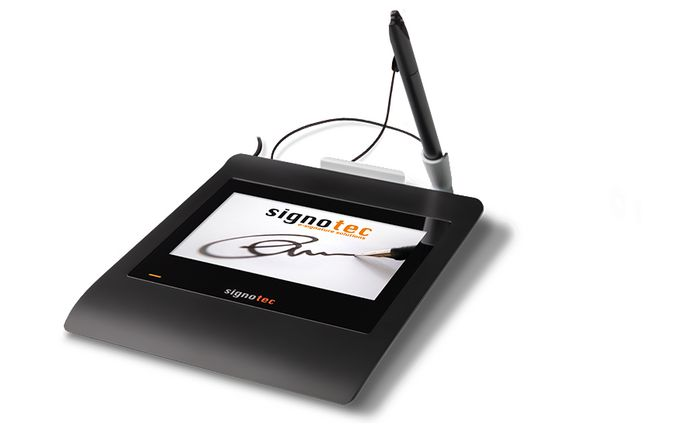
\includegraphics[width=0.5\textwidth]{obrazky-figures/signpad.jpg}
  \caption{signpad.~\cite{SignPadImage}} % https://www.eetgroup.com/cs-cz/st-gert-3-uft100-signotec-signpad-gamma-inkl-ftdi-5in-color-tft-wid-w124375514
  \label{fig:signpad}
\end{figure}

Obecně lze k zaznamenání podpisu také využít tablet s digitálním perem či mobilní telefon.

\subsection*{Algoritmy}
%TODO
Pro proces porovnávání předloženého vzoru a referenčního vzoru uloženého v databázi lze využít několika algoritmů.

\begin{itemize}
  \item \textbf{algoritmus založený na VQ (Vectoral Quantiziation)}
  \item \textbf{algoritmus založený na NN (Nearest Neighbor)}
  \item \textbf{DTW (Dynamic Time Warping)}
  \item \textbf{HMM (Hidden Markov Model)}
\end{itemize}
\noindent
Poté lze tyto algoritmy kombinovat:
\begin{itemize}
  \item \textbf{DTW(VQ)} --- DTW dosáhlo nejlepších výsledků mezi ostatními algoritmy, avšak není použitelný pro vzdálené aplikace, jelikož obsahuje podpis, který je citlivým osobním údajem.
  Není tedy za potřebí posílat celý podpis, ale pouze jeho extahované charakteristiky.
  V ten moment přichází VQ algoritmus. Nejdříve je tedy využit VQ algoritmus a poté je využit DTW algoritmus nad již vektorově kvantizovanými příznakovými vektory.~\cite{Jain2006}
\end{itemize}
% https://www.sciencedirect.com/science/article/abs/pii/S0031320306002780

\subsection*{Důvěryhodnost podpisu}
Nedávné mezinárodní soutěže využívající standardní databáze a testovací protokoly přinesly zajímavé výsledky.   % |
Ukázalo se, že systémy pro ověřování podpisů dosahují vysoké přesnosti.                                         % V
Tato úroveň přesnosti je srovnatelná s jinými pokročilými biometrickými technologiemi.~\cite{Impedovo2008}      % C. Vielhauer, “A behavioural biometrics,” Public Service Rev.: Eur.Union, vol. 20, no. 9, pp. 113–115, 2005.

Experiment se zabýval autenticitou dynamického biometrického podpisu.
V experimentu došli k závěru, že podpis nelze padělat bez znalosti samotného průběhu podpisu.~\cite{6986974} % https://ieeexplore-ieee-org.ezproxy.lib.vutbr.cz/stamp/stamp.jsp?tp=&arnumber=6986974

Následně stejná skupina provedla experiment, kde sstudentům umožnili studovat průběh podpisu.
Závěr byl, že pokud by padělatel měl nejlepší podmínky, tedy možnost zkoumat a replikovat dynamický biometrický podpis jiné osoby bez omezení, 
nemůžeme úspěšné padělání zcela vyloučit, ale pravděpodobnost, že se tak stane, je velmi nízká.~\cite{8585636} % https://ieeexplore-ieee-org.ezproxy.lib.vutbr.cz/stamp/stamp.jsp?tp=&arnumber=8585636

Na závěr tedy můžeme říct, že nejdůležitější však je, že rizikům spojeným s použitím dynamického biometrického podpisu v různých situacích lze vcelku dobře 
předejít volbou správné hranice stupně shody pro akceptaci podpisu.~\cite{8585636} % https://ieeexplore-ieee-org.ezproxy.lib.vutbr.cz/stamp/stamp.jsp?tp=&arnumber=8585636

\section{Hodnocení výhod a nevýhod existujících řešení}
\subsection*{Výhody}
Jednou z hlavních výhod je, že podpis je používán již staletí a je tedy vysoce sociálně akceptovaný, přinejmenším v poměru s jinými biometrickými metodami.
Mezi další výhody pak nadále můžeme například zařadit:

\begin{itemize}
  \item nízkou míru chybovosti falešných odmítnutí či falešných akceptací,
  \item získání obrazu podpisu nemožňuje replikovat dynamické vlastnosti podpisu,
  \item vcelku nízké nároky na uchování podpisu,
  \item levný hardware pro snímaní charakteristik podpisu.
\end{itemize}

\subsection*{Nevýhody}
Mezi nevýhody lze pak zařadit například ovlivnění podpisu i psychickým stavem jedince.
Proto například stres či jiné rozrušení může ovlivnit podpis do takové míry, že dojde k jeho odmítnutí.
Dále může dojít k odmítnutí u osob s nekonzistentním podpisem nebo u jedinců, kterým nějaká nemoc či úraz ovlivnil písmo.

\section{Výběr senzorů a technologií}
Výběr senzorů pro nasnímání dynamických parametrů byl složitý vzhledem k rozměru pera a omezenému rozpočtu. % |
Dalším parametrem hrajícím roli při rozhodování byla přesnost jednotlivých komponent.                       % V
Bylo důležité brát v potaz i to, zda jsou všechny komponenty kompatibilní s použitým mikrořadičem.          % vlatní kec

\subsection*{ESP32}
Mikrořadič ESP32 je jedním z nejrozšířenějších mikrořadičů používaných ve světě.                            % |
V tomto projektu je osazen na vývojové desce ESP32 DevKitC od firmy Espressif.                              % V
Ta je jednou z nejpopulárnějších vývojových desek založených na mikrořadiči ESP32.~\cite{Kolban2017}        % The Official ESP32 book (str. 35)

Vývojová deska ESP32 DevKitC zde slouží jako mozek celého snímání.                                          % |
Jsou k ní připojené všechny ostatní komponenty, které právě mikrořadiči odesílají nasnímaná data.           % V
ESP32 poté tyto data zpracovává a odesílá je do počítače, ke kterému je připojen  pomocí USB kabelu.        % vlastní kec

\subsection*{MPU-6050 (akcelerometr a gyroskop)}
MPU-60X0 je první integrované zařízení na světě pro sledování pohybu v šesti osách pomocí           % |
kombinace tříosého gyroskopu, tříosého akcelerometru a digitálního procesoru pohybu.                % V
Je široce využívaný v mnoha odvětvích, kde je potřeba schopnosti přesně sledovat pohyby uživatele.~\cite{InvenSense2015}% https://invensense.tdk.com/wp-content/uploads/2015/02/MPU-6000-Datasheet1.pdf

Zde slouží ke stejnému účelu, a to snímaní dat pohybu pera při podpisu.                             % |
Snímaná data jsou odesílána v reálném čase mikrořadiči ESP32.                                       % vlastní kec

\subsection*{Tlakový senzor Interlink Electronics FSR® 400}
Model FSR 400 je jednozónový tlakový senzor, tedy má pouze jednu aktivní měřící plochu.                       % |
Rezistory FSR jsou dvouvodičová zařízení a používají robustní polymerové tlustovrstvé snímače.                % |
Ty s rostoucím tlakem na snímač snižují odpor, lze tedy pomocí protékajícího proudu vypočítat sílu stlačení.  % V
Minimální aktivační síla je 0,1 N a maximální citlivost je do 20 N.~\cite{InterlinkElectronicsFSR400}         % https://www.interlinkelectronics.com/fsr-400


\chapter{Návrh snímacího pera}
Pro nasnímání podpisu bylo potřeba sestrojit speciální pero.                                        % |
Toto pero v průběhu podepisování zaznamenává polohu pera ve trojrozměrném prostoru,                 % |
jeho náklon a tlak vyvíjený perem na papír.                                                         % |
V rámci této práce není důležité, aby tyto snímače a celkový systém byl skrytý před uživatelem.     % |
Šlo tedy pouze o vymodelování pera, do kterého bude možné jednotlivé komponenty uložit.             % |
Komponenty bylo nutné připevnit pevně, aby bylo možné snímat přesné a korektní informace o podpisu. % |
Pokud by jednotlivé komponenty nebyly správně upevněny,                                             % V
mělo by to negativní vliv na nasbírané informace a tedy na celou replikaci podpisu.                 % vlastní kec
 
\section{Schéma a popis schématu}
Návrh snímacího pera~\ref{fig:pero} je navrhnut tak, aby fungoval jako normální pero, 
přičemž bylo možné snímat jeho pohyb a další dynamické vlastnosti.
Toho je dosaženo pomocí připevnění mikrořadiče a ostatních komponent přímo na pero.

\begin{figure}[h]
  \centering
  
\includegraphics[width=0.5\textwidth]{obrazky-figures/placeholder.pdf}
  \caption{Pero} 
  \label{fig:pero}
\end{figure}

Do pera je možné uložit jak samotný mikrořadič ESP32~(1), akcelerometr a gyroskop na čipu MPU-6050~(2) tak i tlakové snímače FSR-400.
Tyto tlakové snímače jsou rozmístěny tak, aby se podařilo zachytit co nejvíce informací o tlaku.
Jeden je tedy umístěn nad samotnou náplní propisky, nejvíce využit při psaní kolmo~(3).
Tři další jsou poté rozmístěny u hrotu propisky pro přesnější snímání v případě náklonu pera v průběhu podpisu~(4). 


\section{Možnosti replikace podpisu}
Replikovat podpis, neboli vytvořit falzifikát, lze několika způsoby:

\begin{itemize}
  \item \textbf{Vlastnoruční replikace} --- 
  Napodobení samotného statického podpisu je obtížné, avšak ne nemožné. 
  Bavíme-li se pak o dynamickém podpisu, vytvoření takového falzifikátu se stává nemožným.

  \item \textbf{3D tiskárna} ---
  Napodobit dynamický podpis pomocí 3d tiskárny je možné, ale ve značně omezené míře.
  Lze napodobit rychlost psaní a tlak pera. 
  Napodobení dalších charakteristik, jako je například sklon pera, už pomocí 3d tiskárny nelze.

  \item \textbf{Robotická ruka} ---
  Robotická ruka by měla zvládnout napodobit všechny zaznamenané dynamické údaje o podpisu včetně náklonu pera.
  Mělo by tedy jít o nejlepší dostupnou variantu pro vytvoření důvěryhodného falzifikátu. 
\end{itemize}

\chapter{Závěr}
Tímto bylo probrána všechna potřebná teorie pro pochopení tématu.
Nyní bude potřeba pomocí 3d tisku vytisknout a případně upravit návrh pera.
Vymyslet zapojení periferií, jejich napájení k mikrokontroléru a následné uložení do pera.
Poté naprogramovat kód mikrokontroléru tak, aby odesílal snímaná data přes USB kabel do počítače, kde se budou data ukládat.
Dále nad uloženými daty provést potřebné výpočty a tato upravená data převést na kód pro ovládání robotické ruky.
Následovným testováním a porovnáváním dosáhnout co nejlepších výsledků při tvorbě falzifikátu.
Pomocí speciálního pera by šlo opět nasnímat průběh podpisu, tentokrát vytvořeného robotickou rukou, a tato data mezi sebou porovnávat.
Toto by měl být celý následující postup pro replikaci dynamického podpisu.


%\chapter{Implementace prototypu}
%\section{Vývoj hardwaru}
%\section{Sbírání dat v~reálném čase}
%\section{Ukládání dat pro následnou replikaci podpisu}

%\chapter{Replikace podpisu}
%\section{Využití robotické ruky}
%\section{Transformace nasnímaných dat na kód pro replikaci}
%\section{Testování a výsledky replikace}

%\chapter{Hodnocení výsledků}
%\section{Analýza dosažených výsledků}
%\section{Porovnání s~očekáváními}
%\section{Diskuze o~spolehlivosti a přesnosti replikace}

%\chapter{Závěr}
%\section{Shrnutí hlavních poznatků}
%\section{Zhodnocení významu práce}
%\section{Budoucí perspektivy}

%\section{Možná vylepšení a rozšíření}
%\*subsection{Návrhy na zlepšení prototypu}
%\*subsection{Možnosti dalšího výzkumu a vývoje}


%===============================================================================

% Pro kompilaci po částech (viz projekt.tex) nutno odkomentovat
%\end{document}
